\documentclass{beamer}
%\usepackage{beamerthemeAmsterdam}
\usepackage{amsmath}
\usepackage{graphicx}

\usepackage{color}
\usepackage{hyperref}
\hypersetup{linkcolor=blue,filecolor=red}

\title{JPEG-2000}
\subtitle{De Wondere Wereld van Wavelets}
\author{Jan Westerdiep \and Okke van Garderen}
\date{\today}
\institute{Universiteit van Amsterdam}

\begin{document}

\frame{\titlepage}

\section{Intro}
\frame{
  \frametitle{Vakantieplaatje}
  \begin{columns}
    \begin{column}{0.5\textwidth}
      \hfill
      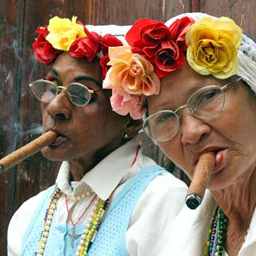
\includegraphics[width=\textwidth]{cigar.png}
      \hfill
    \end{column}
    \pause
    \begin{column}{0.5\textwidth}
      \hfill
      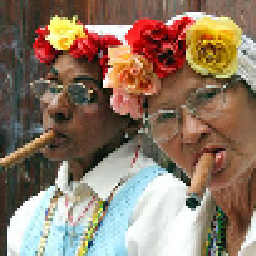
\includegraphics[width=\textwidth]{cigar_downscale.png}
      \hfill
    \end{column}
  \end{columns}
}
\frame{
  \frametitle{Vakantieplaatje}
  \begin{columns}
    \begin{column}{0.5\textwidth}
      \hfill
      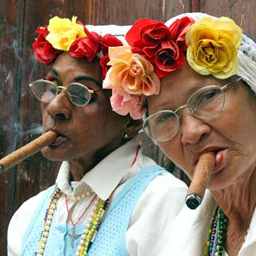
\includegraphics[width=\textwidth]{cigar.png}
      \hfill
    \end{column}
    \begin{column}{0.5\textwidth}
      \hfill
      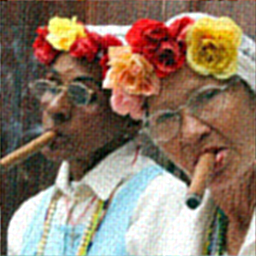
\includegraphics[width=\textwidth]{cigar_fourier.png}
      \hfill
    \end{column}
  \end{columns}
}
\frame{
  \frametitle{Vakantieplaatje}
  \begin{columns}
    \begin{column}{0.5\textwidth}
      \hfill
      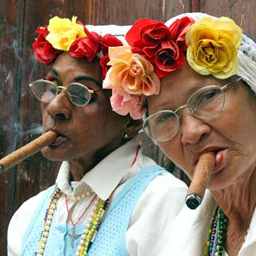
\includegraphics[width=\textwidth]{cigar.png}
      \hfill
    \end{column}
    \begin{column}{0.5\textwidth}
      \hfill
      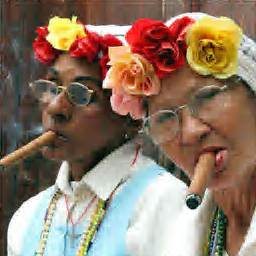
\includegraphics[width=\textwidth]{cigar_db2.png}
      \hfill
    \end{column}
  \end{columns}
}

\frame{
	\frametitle{Ons project}
	\begin{itemize}
		\item Beeldcompressie
		\item JPEG: Fouriertransformatie
		\item JPEG-2000: Wavelettransformatie
	\end{itemize}
}

\frame{
	\frametitle{Fouriertransformatie}
	\begin{itemize}
	\item Beginsignaal $f$
	\item Transformatie is omschrijven naar andere basis 
          \[
          f(x) = \sum_k a_k \cos(k x) + b_k \sin(k x)
          \]
	\item Compressie door minst significante termen weg te laten
	\item Nadeel: werkt niet goed bij plaatjes met scherpe randen
	\end{itemize}
\pause
        
\includegraphics[width=0.25 \textwidth]{sin.png}
        
\includegraphics[width=0.25 \textwidth]{sin_fourier.pdf}
        
\includegraphics[width=0.25 \textwidth]{smiley.png}
        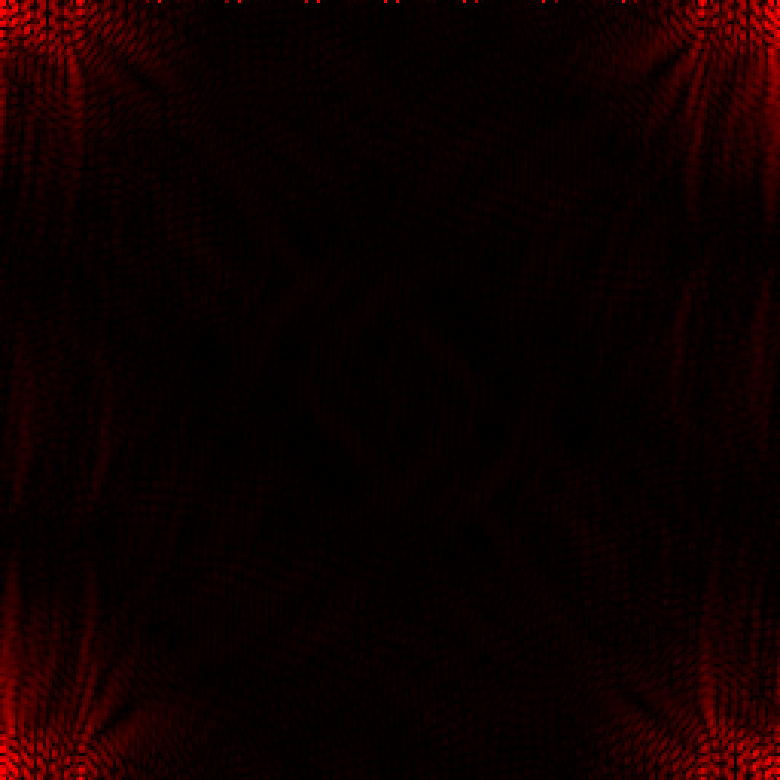
\includegraphics[width=0.25 \textwidth]{smiley_fourier.pdf}
}

\frame{
	\frametitle{Wavelettransformatie}
	\begin{columns}
		\begin{column}{0.5\textwidth}
			\begin{itemize}
				\item Weer omschrijven in een andere basis
				\item Heel veel soorten wavelets
				\item Jong onderzoeksgebied dus er is nog veel te ontdekken
				\item Randen zijn alleen lokaal zichtbaar $\implies$ betere compressie
			\end{itemize}
		\end{column}
		\begin{column}{0.5\textwidth}
			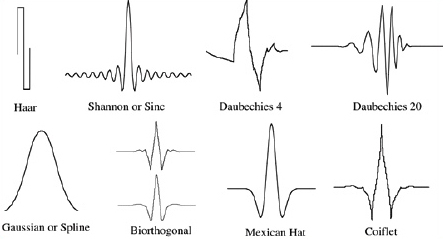
\includegraphics[width=\textwidth]{wavelets.jpg}\\
			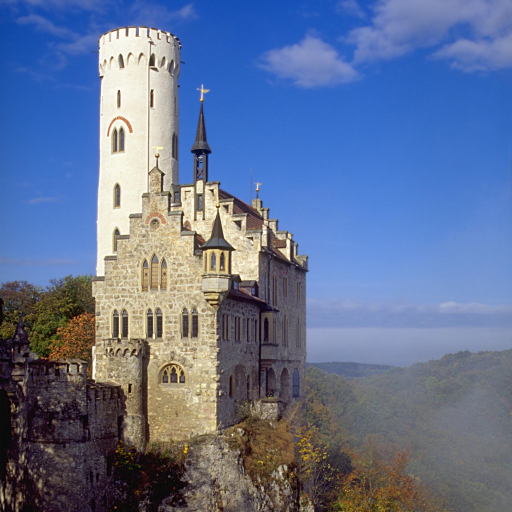
\includegraphics[width=0.5\textwidth]{huis.png}
			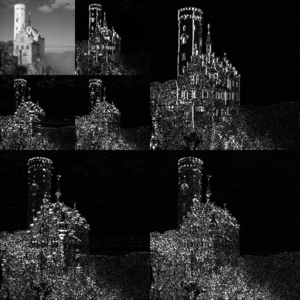
\includegraphics[width=0.5\textwidth]{huis_wavelet_transformed.png}
		\end{column}
	\end{columns}
}
\frame{
  \frametitle{Lenna}
  \vspace{18pt}
  \centering \hspace{-0.5px}~~~~~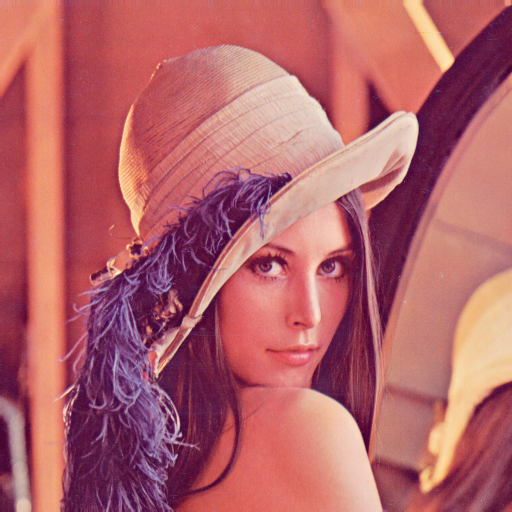
\includegraphics[height=0.72\textheight]{Lenna.png}
}

\frame{
	\frametitle{Voorbeelden (1\%)}
  \begin{table}
    \begin{tabular}{c c c c}
      Downscale &
      
\includegraphics[width=0.3\linewidth]{Lenna_downscale.png} &
      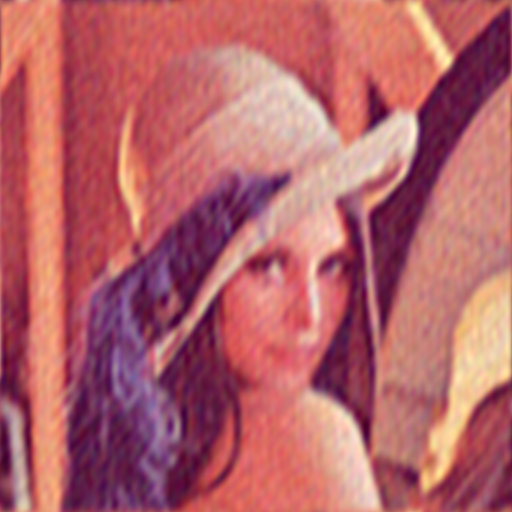
\includegraphics[width=0.3\linewidth]{Lenna_fourier.png} &
      Fourier \\
      Haar &
      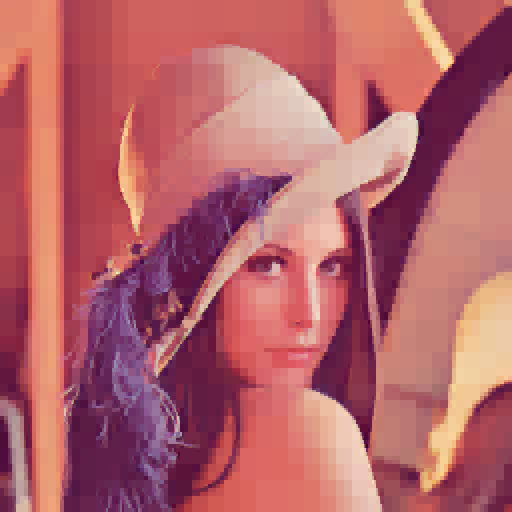
\includegraphics[width=0.3\linewidth]{Lenna_haar.png} &
      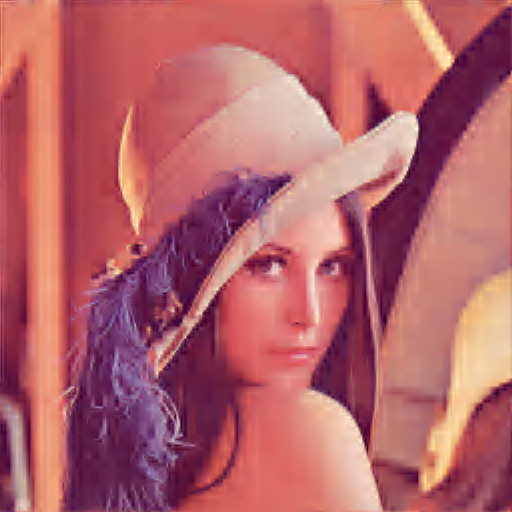
\includegraphics[width=0.3\linewidth]{Lenna_db2.png} &
      Daubechies 2
    \end{tabular}
  \end{table}
}

\frame{
	\frametitle{Filmpjes (2\%)}
        \href{pag6b.html}{Link naar gifjes}
}

\frame{
  \begin{table}
    \begin{tabular}{r c c l}
      Origineel &
      
\includegraphics[width=0.3\linewidth]{gentoo.png} &
      
\includegraphics[width=0.3\linewidth]{gentoo_new_1p.png} &
      Fourier \\
      Haar &
      
\includegraphics[width=0.3\linewidth]{gentoo_01_haar_smooth.png} &
      
\includegraphics[width=0.3\linewidth]{gentoo_01_db2_smooth.png} &
      Daubechies 2
    \end{tabular}
  \end{table}
}

\end{document}
